\section{gyro\_\-spi.c File Reference}
\label{gyro__spi_8c}\index{gyro_spi.c@{gyro\_\-spi.c}}
{\tt \#include $<$inttypes.h$>$}\par
{\tt \#include $<$avr/io.h$>$}\par
{\tt \#include $<$avr/interrupt.h$>$}\par
{\tt \#include \char`\"{}gyro\_\-spi.h\char`\"{}}\par
{\tt \#include \char`\"{}globals.h\char`\"{}}\par


Include dependency graph for gyro\_\-spi.c:\begin{figure}[H]
\begin{center}
\leavevmode
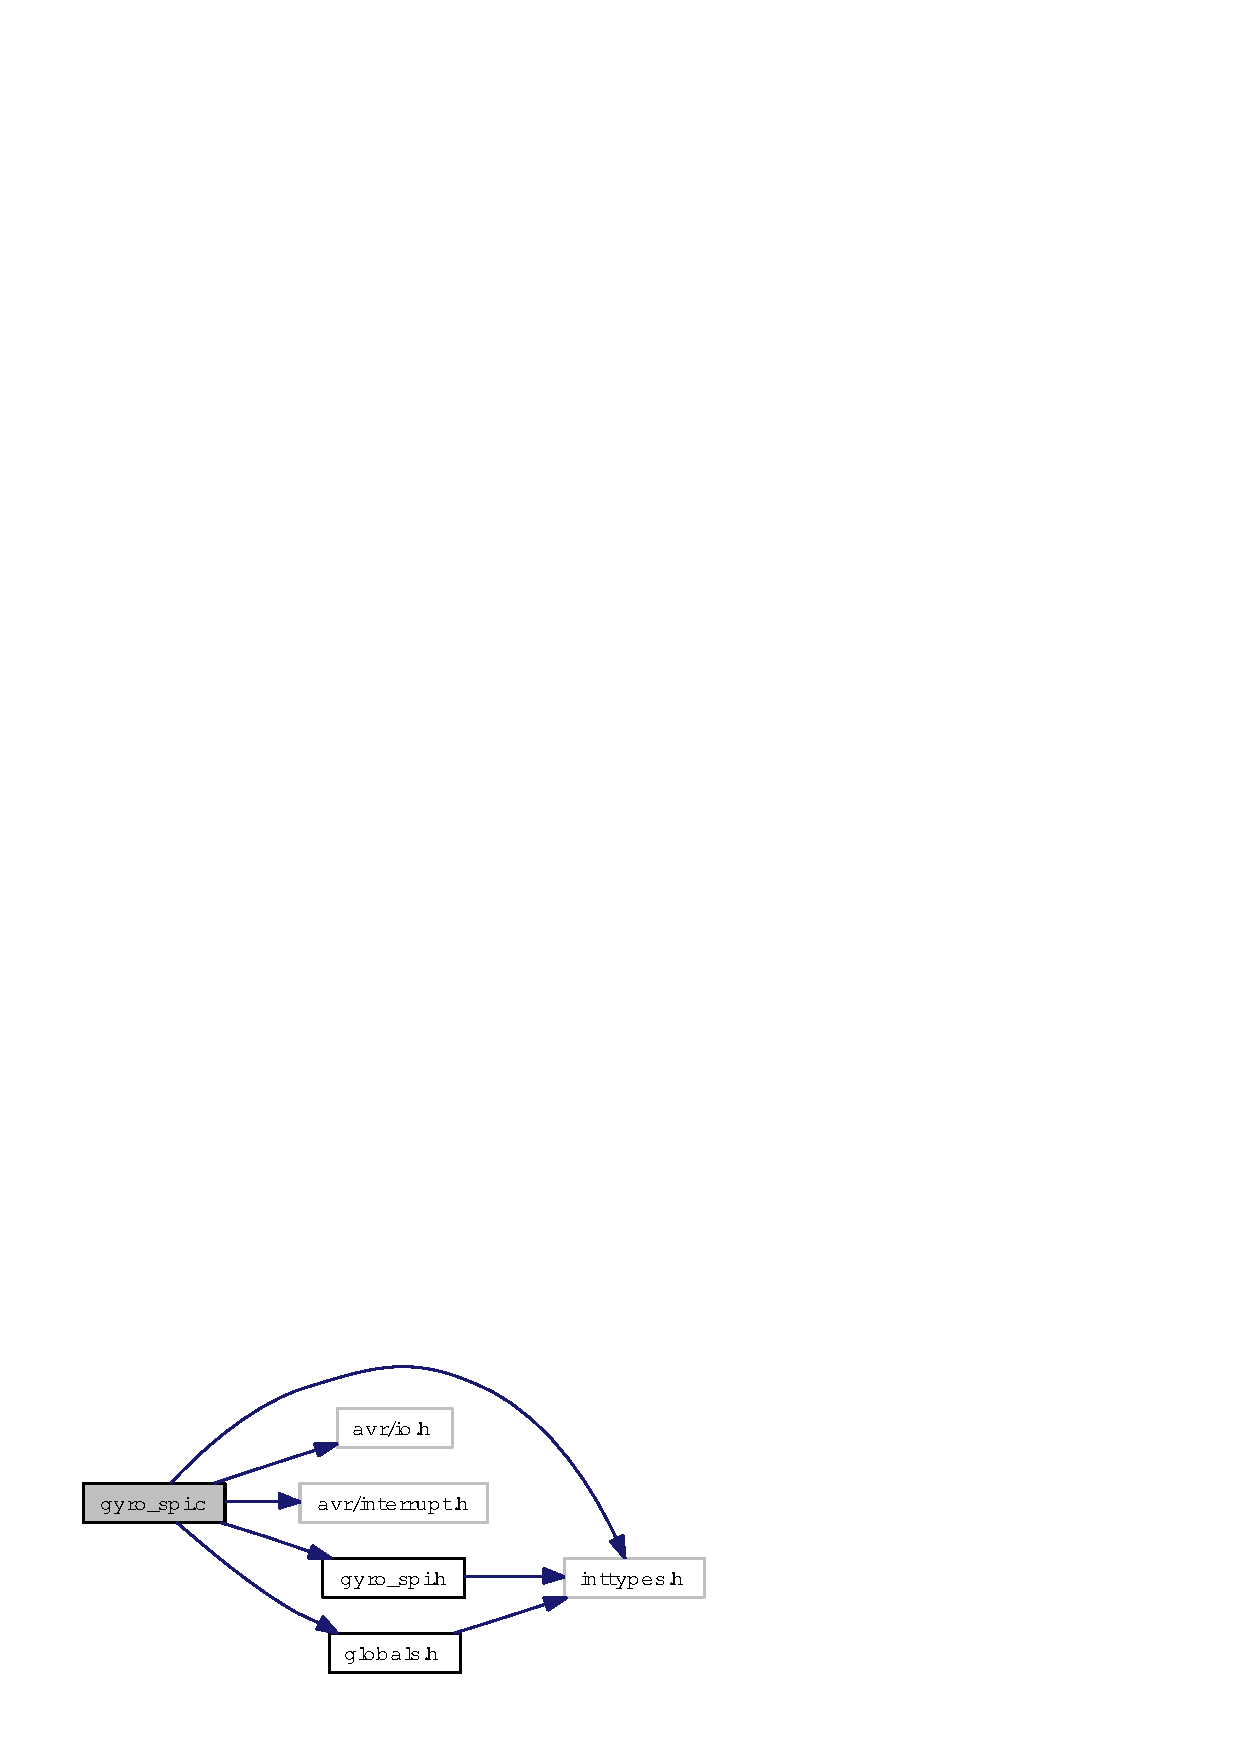
\includegraphics[width=171pt]{gyro__spi_8c__incl}
\end{center}
\end{figure}
\subsection*{Functions}
\begin{CompactItemize}
\item 
{\bf SIGNAL} (SIG\_\-SPI)
\item 
void {\bf init\_\-spi\_\-gyro} (uint8\_\-t interrupt\_\-mode)
\item 
void {\bf spi\_\-cs} (uint8\_\-t chip)
\item 
uint8\_\-t {\bf spi\_\-write\_\-8} (uint8\_\-t data)
\begin{CompactList}\small\item\em Transfer 1 Byte given in data via the SPI return the 1 Byte sampled during transfer. \item\end{CompactList}\item 
uint8\_\-t {\bf spi\_\-write\_\-8\_\-nocs} (uint8\_\-t data)
\item 
uint16\_\-t {\bf spi\_\-write\_\-16} (uint16\_\-t data)
\begin{CompactList}\small\item\em Tranfer 2 Bytes given in data via the SPI, return the 2 Bytes sampled during transfer. \item\end{CompactList}\item 
uint16\_\-t {\bf spi\_\-write\_\-16\_\-nocs} (uint16\_\-t data)
\end{CompactItemize}
\subsection*{Variables}
\begin{CompactItemize}
\item 
uint8\_\-t {\bf highbyte\_\-temp}
\end{CompactItemize}


\subsection{Function Documentation}
\index{gyro_spi.c@{gyro\_\-spi.c}!SIGNAL@{SIGNAL}}
\index{SIGNAL@{SIGNAL}!gyro_spi.c@{gyro\_\-spi.c}}
\subsubsection{\setlength{\rightskip}{0pt plus 5cm}SIGNAL (SIG\_\-SPI)}\label{gyro__spi_8c_734dd027fc9ababff59a6e870ee42a76}


The SPI interrupt service routine. This route is called everytime, a byte has been completly transmitted over the SPI-Interface. According to the current state of the transmission, either the low-byte of the 16bit word has to be send, or a new transfer needs to be started 

Definition at line 66 of file gyro\_\-spi.c.

References ACC\_\-HB, ACC\_\-LB, CS\_\-GYRO2, first\_\-run, g1\_\-hacc, g1\_\-htmp, g1\_\-lacc, g1\_\-ltmp, g2\_\-hacc, g2\_\-htmp, g2\_\-lacc, g2\_\-ltmp, gyro1\_\-idx, gyro1\_\-samples, GYRO1\_\-SAMPLES\_\-BUFSIZE, gyro1\_\-temp, gyro2\_\-idx, gyro2\_\-samples, GYRO2\_\-SAMPLES\_\-BUFSIZE, gyro2\_\-temp, gyro\_\-state, highbyte\_\-temp, read\_\-gyro\_\-temp, TEMP\_\-HB, and TEMP\_\-LB.

\subsection{Variable Documentation}
\index{gyro_spi.c@{gyro\_\-spi.c}!highbyte_temp@{highbyte\_\-temp}}
\index{highbyte_temp@{highbyte\_\-temp}!gyro_spi.c@{gyro\_\-spi.c}}
\subsubsection{\setlength{\rightskip}{0pt plus 5cm}uint8\_\-t {\bf highbyte\_\-temp}}\label{gyro__spi_8c_a1d7fd7792fd6135e91c3228ff8cc102}




Definition at line 58 of file gyro\_\-spi.c.

Referenced by SIGNAL().